\subsubsection*{Analysis}
\begin{tabular}{@{}l l}
\textbf{Scope}:&The AuctionHouse\textsuperscript{TM} automated administration system\\
\textbf{Level}:&User goal\\
\textbf{Primary Actor}:&Owner \& Secretary\\
\textbf{Stakeholders and Interests}:&\begin{tabular}[t]{@{}l}Owner: wants to register his staff to the system.\\Secretary: wants to register buyers and sellers to the system.\\Staff, Buyers and Sellers: Want to be granted access to the system.\end{tabular}\\
\textbf{Preconditions}:&User is identified and authenticated.\\
\textbf{Postconditions}:&\begin{tabular}[t]{@{}l}A new user has been registered to the system.\\The person for whom a new user has been added received\\the necessary authorization credentials for the system.\end{tabular}\\
\textbf{Special requirements}:&A list of categories and a list of future auction dates needs to available in the system\\
\textbf{Frequency of occurence}:& \begin{tabular}[t]{@{}l}Depedent on the amount of job applications and new buyers and sellers per month.\\Since not many staff members at required, the former will be rare, say 1 per month.\\The latter will be more common, say 10 times per month. That is an estimated\\11 times per month.\end{tabular}
\end{tabular}\\\\
\textsl{Main Success Scenario}
\begin{enumerate}[noitemsep]
	\item The user starts the `add user' transaction with the system, having all parameters of the user to be added ready.
	\item The system confirms the interaction and asks the user to provide all the necessary parameters.
	\item The user provides all necessary parameters. The parameters to provide are (optional parameters are marked with a `*'):
	\begin{itemize}[noitemsep]
		\item The name of the new user (username)
		\item The class of the new user (e.g. Staff member, Buyer, Seller)\\
		\quad The selection depends on the user doing the transaction
		\item The address of the person bound to the new user
		\item * An email address (for digital mail)
		\item * A bank account number for deposits/sallary
	\end{itemize}
	\item The system creates the user with all provided parameters and adds it to the list. It also generates authentication credentials for the person bound to the new user.
	\item The system returns to the user with a confirmation message containing the generated authentication credentials, or a failure.
\end{enumerate}
\textsl{Extensions}
\begin{itemize}[noitemsep]
	\item When a failure is returned, the system state remains unchanged; no user or other parameters was added.
	\item When not all required parameters were provided, the system will first ask the user to provide it until all parameters is provided.
	\item The system will only provide the classes for the new user based on the class of the user who is doing the transaction.
\end{itemize}
\textsl{System Sequence Diagram}
\begin{figure}[H]
	\centering
	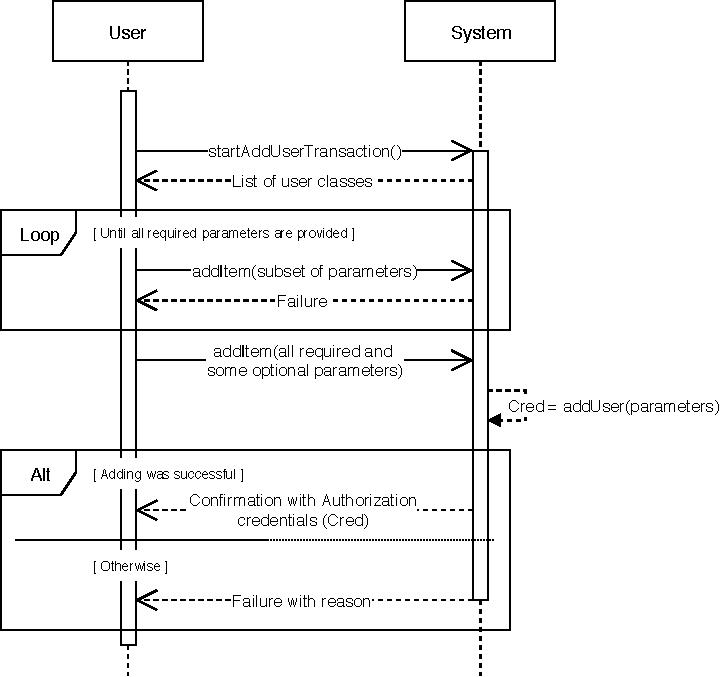
\includegraphics[scale=1]{SD-bb-createuser.pdf}
	\caption*{Interactions displayed in a System Sequence Diagram defined by the MSS and its extensions in blackbox format}
\end{figure}